\section{Combat Modifiers}
Sometimes you just have to go toe-to-toe in a fight, but you can
usually gain some advantage by seeking a better position, either
offensively or defensively. This section covers the rules for when
you can line up a particularly good attack or are forced to make a
disadvantageous one.

\subsection{(Un)Favorable Conditions}
% \subsection{Favorable and Unfavorable Conditions}
Depending on the condition of attackers or defenders, they may gain bonuses or penalties as stated in \tabref{Attack Roll Modifiers} and \tabref{Armor Class Modifiers}.

\Table{Attack Roll Modifiers}{L*{2}{Z{12mm}}}{
\tableheader Attacker is... & \tableheader Melee & \tableheader Ranged\\
Dazzled & $-1$ & $-1$ \\
Entangled & $-2$\footnotemark[1] & $-2$\footnotemark[1] \\
Flanking defender & +2 & --- \\
Invisible & +2\footnotemark[2] & +2\footnotemark[2] \\
On higher ground & +1 & +0 \\
Prone & $-4$ & ---\footnotemark[3] \\
Shaken or frightened & $-2$ & $-2$ \\
Squeezing through a space & $-4$ & $-4$ \\

\TableNote{3}{1 An entangled character also takes a $-4$ penalty to Dexterity, which may affect his attack roll.}\\
\TableNote{3}{2 The defender loses any Dexterity bonus to AC. This bonus doesn't apply if the target is blinded.}\\
\TableNote{3}{3 Most ranged weapons can't be used while the attacker is prone, but you can use a crossbow or shuriken while prone at no penalty.}\\
}

\Table{Armor Class Modifiers}{L*{2}{Z{12mm}}}{
\tableheader Defender is... & \tableheader Melee & \tableheader Ranged\\
Behind cover & +4 & +4 \\
Blinded & $-2$\footnotemark[1] & $-2$\footnotemark[1] \\
Concealed or invisible & \multicolumn{2}{c}{See Concealment} \\
Cowering & $-2$\footnotemark[1] & $-2$\footnotemark[1] \\
Entangled & +0\footnotemark[2] & +0\footnotemark[2] \\
Flat-footed (such as surprised, balancing, climbing) & +0\footnotemark[1] & +0\footnotemark[1] \\
Grappling (but attacker is not) & +0\footnotemark[1] & +0\footnotemark[1]\footnotemark[3] \\
Helpless (such as paralyzed, sleeping, or bound) & $-4$\footnotemark[4] & +0\footnotemark[4] \\
Kneeling or sitting & $-2$ & +2 \\
Pinned & $-4$\footnotemark[4] & +0\footnotemark[4] \\
Prone & $-4$ & +4 \\
Squeezing through a space & $-4$ & $-4$ \\
Stunned & -2\footnotemark[1] & -2\footnotemark[1] \\

\TableNote{3}{1 The defender loses any Dexterity bonus to AC.}\\
\TableNote{3}{2 An entangled character takes a $-4$ penalty to Dexterity.}\\
\TableNote{3}{3 Roll randomly to see which grappling combatant you strike. That defender loses any Dexterity bonus to AC.}\\
\TableNote{3}{4 Treat the defender's Dexterity as 0 ($-5$ modifier). Rogues can sneak attack helpless or pinned defenders.}\\
}

\begin{figure*}[t!]
\centering
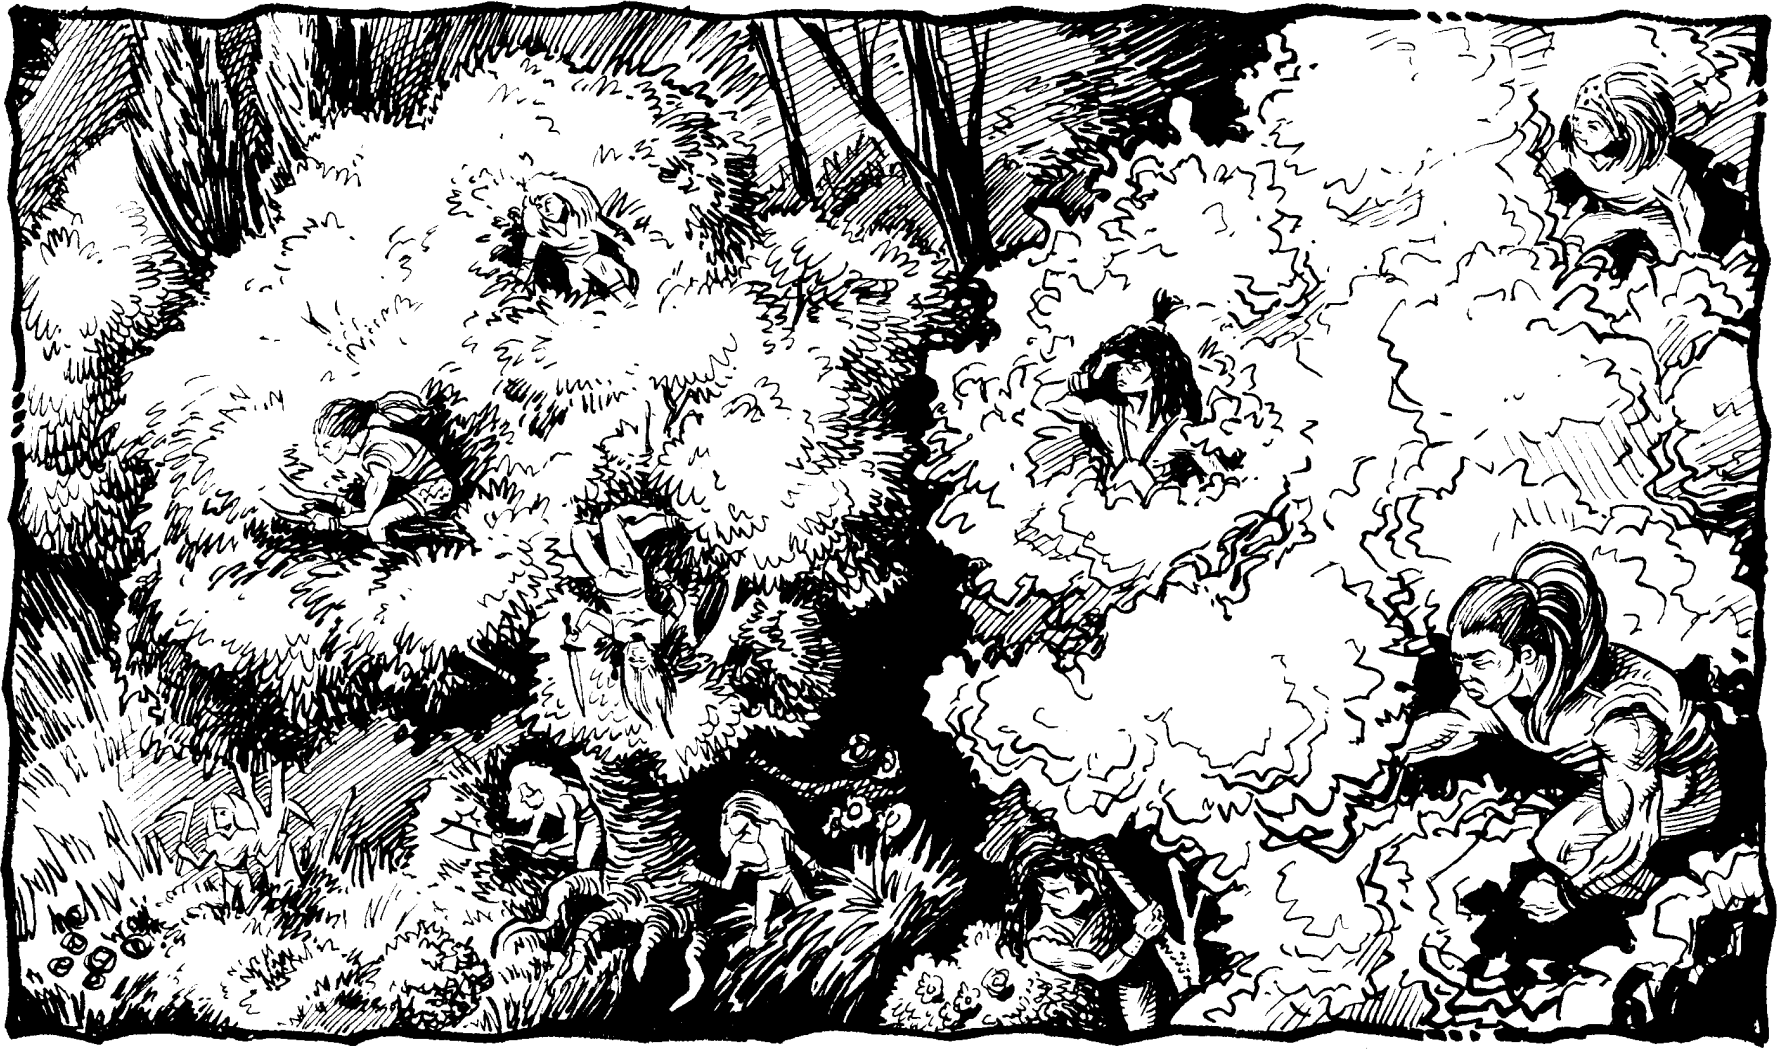
\includegraphics[width=\textwidth]{images/cover-1.png}
\WOTC
\end{figure*}
\subsection{Cover}
To determine whether your target has cover from your ranged attack, choose a corner of your square. If any line from this corner to any corner of the target's square passes through a square or border that blocks line of effect or provides cover, or through a square occupied by a creature, the target has cover (+4 to AC).

When making a melee attack against an adjacent target, your target has cover if any line from your square to the target's square goes through a wall (including a low wall). When making a melee attack against a target that isn't adjacent to you (such as with a reach weapon), use the rules for determining cover from ranged attacks.

\textbf{Low Obstacles and Cover:} A low obstacle (such as a wall no higher than half your height) provides cover, but only to creatures within 9 meters (6 squares) of it. The attacker can ignore the cover if he's closer to the obstacle than his target.

\textbf{Cover and Attacks of Opportunity:} You can't execute an attack of opportunity against an opponent with cover relative to you.

\textbf{Cover and Reflex Saves:} Cover grants you a +2 bonus on Reflex saves against attacks that originate or burst out from a point on the other side of the cover from you. Note that spread effects can extend around corners and thus negate this cover bonus.

\textbf{Cover and Hide Checks:} You can use cover to make a \skill{Hide} check. Without cover, you usually need concealment to make a \skill{Hide} check.

\textbf{Soft Cover:} Creatures, even your enemies, can provide you with cover against ranged attacks, giving you a +4 bonus to AC. However, such soft cover provides no bonus on Reflex saves, nor does soft cover allow you to make a \skill{Hide} check.

\textbf{Big Creatures and Cover:} Any creature with a space larger than 1.5 meter (1 square) determines cover against melee attacks slightly differently than smaller creatures do. Such a creature can choose any square that it occupies to determine if an opponent has cover against its melee attacks. Similarly, when making a melee attack against such a creature, you can pick any of the squares it occupies to determine if it has cover against you.

\textbf{Total Cover:} If you don't have line of effect to your target he is considered to have total cover from you. You can't make an attack against a target that has total cover.

\textbf{Varying Degrees of Cover:} In some cases, cover may provide a greater bonus to AC and Reflex saves. In such situations the normal cover bonuses to AC and Reflex saves can be doubled (to +8 and +4, respectively). A creature with this improved cover effectively gains improved evasion against any attack to which the Reflex save bonus applies. Furthermore, improved cover provides a +10 bonus on \skill{Hide} checks.
\subsection{Concealment}
To determine whether your target has concealment from your ranged attack, choose a corner of your square. If any line from this corner to any corner of the target's square passes through a square or border that provides concealment, the target has concealment.

When making a melee attack against an adjacent target, your target has concealment if his space is entirely within an effect that grants concealment. When making a melee attack against a target that isn't adjacent to you use the rules for determining concealment from ranged attacks.

In addition, some magical effects provide concealment against all attacks, regardless of whether any intervening concealment exists.

\textbf{Concealment Miss Chance:} Concealment gives the subject of a successful attack a 20\% chance that the attacker missed because of the concealment. If the attacker hits, the defender must make a miss chance percentile roll to avoid being struck. Multiple concealment conditions do not stack.

\textbf{Concealment and Hide Checks:} You can use concealment to make a Hide check. Without concealment, you usually need cover to make a Hide check.

\textbf{Total Concealment:} If you have line of effect to a target but not line of sight he is considered to have total concealment from you. You can't attack an opponent that has total concealment, though you can attack into a square that you think he occupies. A successful attack into a square occupied by an enemy with total concealment has a 50\% miss chance (instead of the normal 20\% miss chance for an opponent with concealment).

You can't execute an attack of opportunity against an opponent with total concealment, even if you know what square or squares the opponent occupies.

\textbf{Ignoring Concealment:} Concealment isn't always effective. A shadowy area or darkness doesn't provide any concealment against an opponent with darkvision. Characters with low-light vision can see clearly for a greater distance with the same light source than other characters. Although invisibility provides total concealment, sighted opponents may still make Spot checks to notice the location of an invisible character. An invisible character gains a +20 bonus on Hide checks if moving, or a +40 bonus on Hide checks when not moving (even though opponents can't see you, they might be able to figure out where you are from other visual clues).

\textbf{Varying Degrees of Concealment:} Certain situations may provide more or less than typical concealment, and modify the miss chance accordingly.
\subsection{Flanking}
When making a melee attack, you get a +2 flanking bonus if your opponent is threatened by a character or creature friendly to you on the opponent's opposite border or opposite corner.

When in doubt about whether two friendly characters flank an opponent in the middle, trace an imaginary line between the two friendly characters' centers. If the line passes through opposite borders of the opponent's space (including corners of those borders), then the opponent is flanked.

\textit{Exception:} If a flanker takes up more than 1 square, it gets the flanking bonus if any square it occupies counts for flanking.

Only a creature or character that threatens the defender can help an attacker get a flanking bonus.

Creatures with a reach of 0 feet can't flank an opponent.
\subsection{Helpless Defenders}
A helpless opponent is someone who is bound, sleeping, paralyzed, unconscious, or otherwise at your mercy.

\textbf{Regular Attack:} A helpless character takes a $-4$ penalty to AC against melee attacks, but no penalty to AC against ranged attacks.

A helpless defender can't use any Dexterity bonus to AC. In fact, his Dexterity score is treated as if it were 0 and his Dexterity modifier to AC as if it were $-5$ (and a rogue can sneak attack him).

\textbf{Coup de Grace:} As a full-round action, you can use a melee weapon to deliver a coup de grace to a helpless opponent. You can also use a bow or crossbow, provided you are adjacent to the target.

You automatically hit and score a critical hit. If the defender survives the damage, he must make a Fortitude save (DC 10 + damage dealt) or die. A rogue also gets her extra sneak attack damage against a helpless opponent when delivering a coup de grace.

Delivering a coup de grace provokes attacks of opportunity from threatening opponents.

You can't deliver a coup de grace against a creature that is immune to critical hits. You can deliver a coup de grace against a creature with total concealment, but doing this requires two consecutive full-round actions (one to ``find'' the creature once you've determined what square it's in, and one to deliver the coup de grace).

\subsection{Weapon, Armor, and Shield Proficiency}
A character who uses a weapon with which he or she is not proficient takes a $-4$ penalty on attack rolls.

A character who wears armor and/or uses a shield with which he or she is not proficient takes the armor's (and/or shield's) armor check penalty on attack rolls and on all Strength-based and Dexterity-based ability and skill checks. The penalty for nonproficiency with armor stacks with the penalty for nonproficiency with shields

Weapon, armor, or shield proficiency may be granted by the character's race, class or by the following feats:

\begin{itemize*}
\item \feat{Armor Proficiency (Light)}
\item \feat{Armor Proficiency (Medium)}
\item \feat{Armor Proficiency (Heavy)}
\item \feat{Exotic Weapon Proficiency}
\item \feat{Martial Weapon Proficiency}
\item \feat{Shield Proficiency}
\item \feat{Simple Weapon Proficiency}
\item \feat{Tower Shield Proficiency}
\end{itemize*}
